\chapter{A framework for streaming analysis of short DNA sequencing reads based
on k-mer counting}

\section{Introduction}

In last chapter, we introduced an efficient k-mer counting approach based on a
probabilistic data structure. In this chapter, we will discuss the application
of this approach to enable streaming analysis of short DNA sequencing reads.
First, we will show a novel approach to use median k-mer count in a read to estimate
sequencing depth without a reference assembly. Next based on this approach two
streaming methods that are critically important in next generation sequencing
data analysis will be discussed. One is the single-pass method to eliminate redundant reads in
data sets to reduce computational cost in down-streaming analysis like
assembly, which is termed as "digital normalization". The other one is the
method to analyze and trim sequencing errors in short reads dat asets, in a
semi-streaming or streaming fashion.

The approach to use median k-mer count to estimate sequencing depth of a read is
also the foundation of the IGS based diversity analysis approach we will
discuss in the next chapter. The streaming methods to remove redundant reads
and sequencing error analysis and trimming are not directly related to the IGS
based diversity analysis method, nevertheless the applications of the two
streaming methods to facilitate the assembly of metagenomic reads and remove
sequencing errors in reads data sets benefit many bioinformatics approaches,
including the microbial diversity analysis.
% 
% % % 
\section{Estimating sequencing depth without a reference assembly}

Short-read assembly requires deep sequencing to systematically sample the
source genome, because shotgun sequencing is subject to both random sampling
variation and systematic sequencing biases.  For example, 100x sampling of a
human genome is required for recovery of 90\% or more of the genome in contigs
$>$ 1kb \cite{pubmed21187386}. In principle much of this high-coverage data is
redundant and could be eliminated without consequence to the final assembly,
but determining which reads to eliminate requires a per-read estimate of
coverage. Traditional approaches estimate coverage by mapping reads to an
assembly.  This presents a chicken-and-egg problem: to determine which regions
are oversampled, we must already have an assembly!

\begin{figure}[!ht]
\centerline{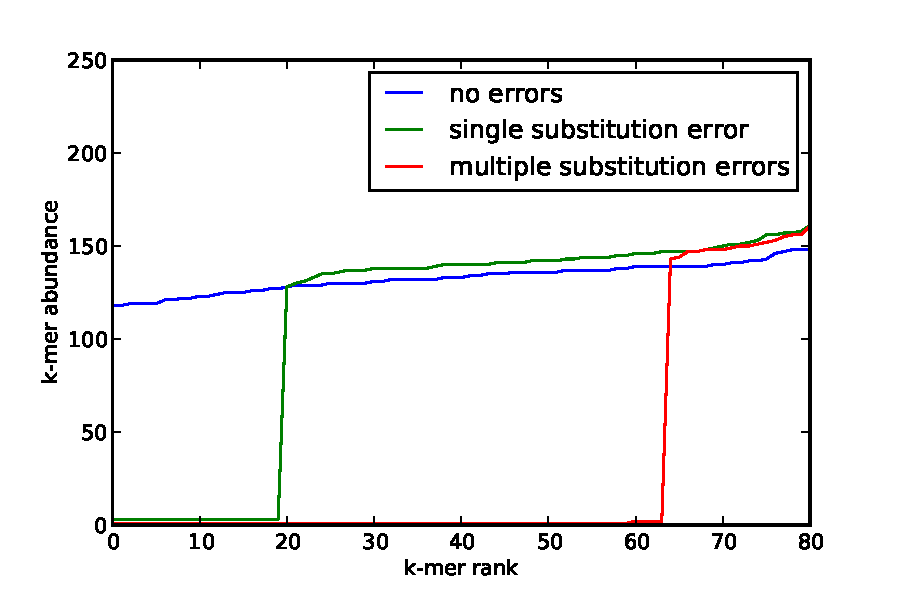
\includegraphics[width=4in]{diginorm-ranks.pdf}} \caption{ {\bf
Representative rank-abundance distributions for 20-mers from 100-base reads
with no errors, a read with a single substitution error, and a read with
multiple substitution errors.}} \label{fig:rankabund} \end{figure}

We may calculate a {\em reference-free} estimate of genome coverage by looking
at the k-mer abundance distribution within individual reads. First, observe
that k-mers, DNA words of a fixed length $k$, tend to have similar abundances
within a read: this is a well-known property of k-mers that stems from each
read originating from a single source molecule of DNA.  The more times a region
is sequenced, the higher the abundance of k-mers from that region would be.  In
the absence of errors, average k-mer abundance could be used as an estimate of
the depth of coverage for a particular read (Figure \ref{fig:rankabund}, ``no
errors'' line).  However, when reads contain random substitution or indel
errors from sequencing, the k-mers overlapping these errors will be of lower
abundance; this feature is often used in k-mer based error correction
approaches \cite{pubmed21114842}.  For example, a single substitution will
introduce $k$ low-abundance k-mers within a read.  (Figure \ref{fig:rankabund},
``single substitution error'' line).  However, for small $k$ and reads of
length $L$ where $L > 3k-1$, a single substitution error will not skew the {\em
median} k-mer abundance.  Only when multiple substitution errors are found in a
single read will the median k-mer abundance be affected (Figure
\ref{fig:rankabund}, ``multiple substitution errors''). The effect of multiple
errors to median k-mer abundance will be discussed in details in next chapter.


\begin{figure}[!ht] \begin{center}
\centerline{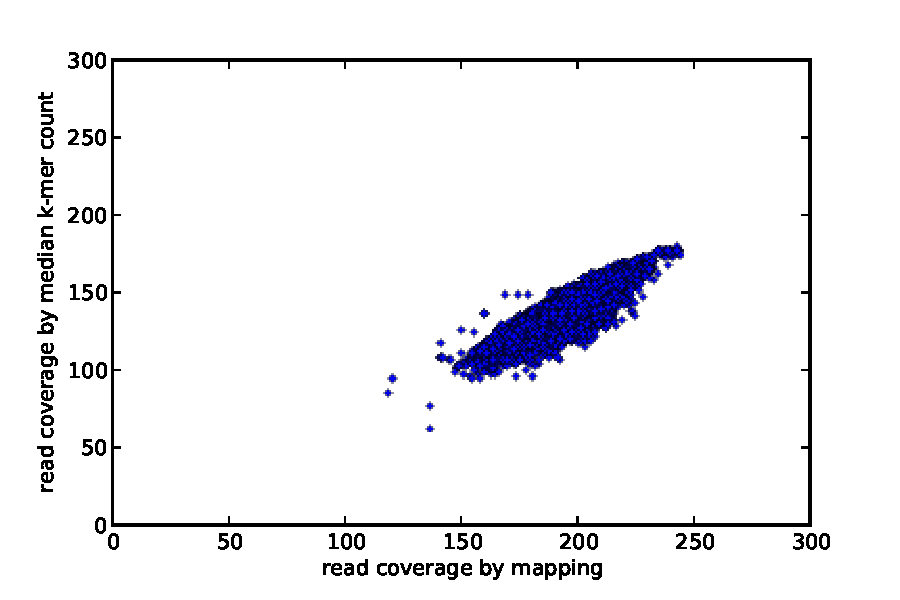
\includegraphics[width=3in]{diginorm-sim-genome.pdf}}
\centerline{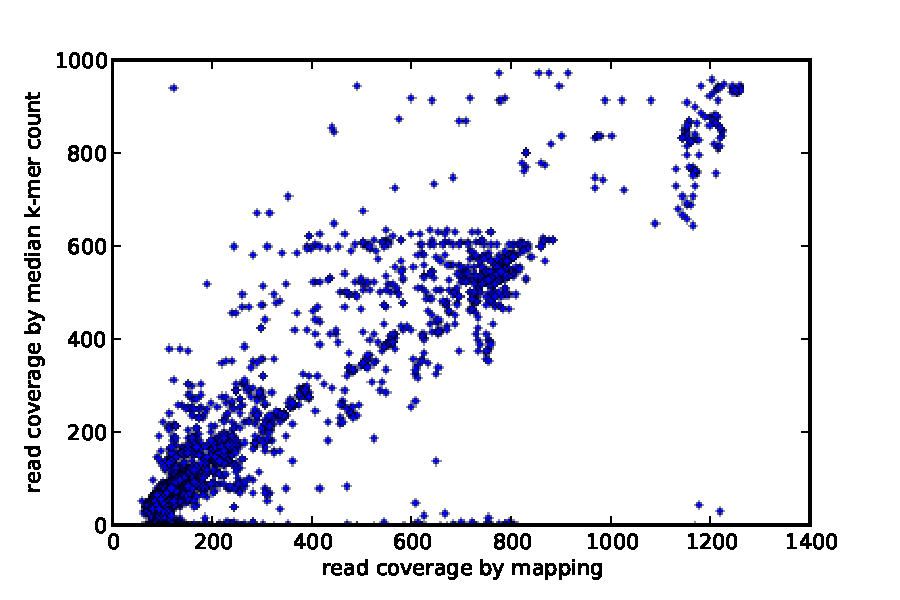
\includegraphics[width=3in]{diginorm-ecoli-genome.pdf}}
\end{center} \caption{ {\bf Mapping and k-mer coverage measures correlate for
simulated genome data and a real {\em E. coli} data set (5m reads).  Simulated
data $r^2 = 0.79$; {\em E. coli} $r^2 = 0.80$.}
}
\label{fig:random} \end{figure}


\begin{figure}[!ht] \begin{center}
\centerline{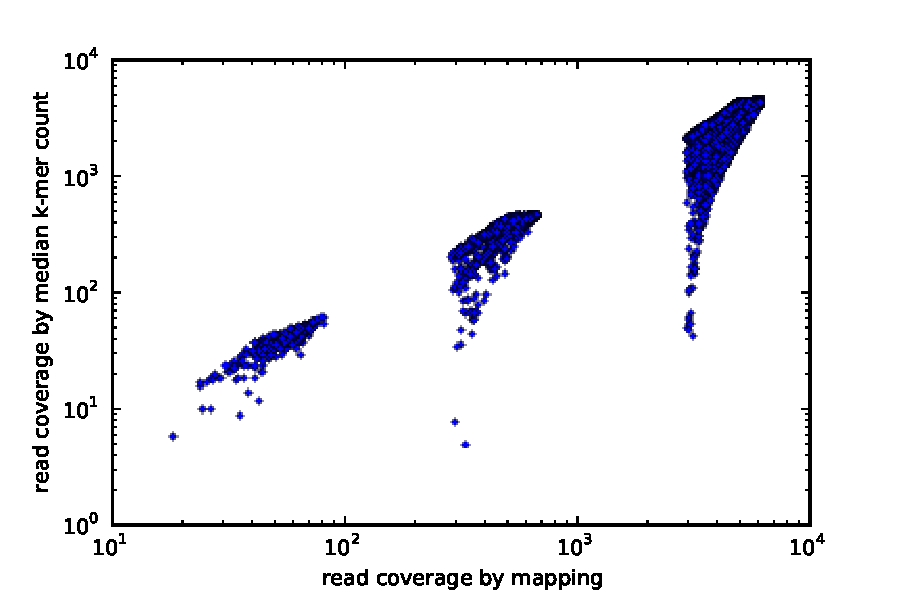
\includegraphics[width=3in]{diginorm-sim-transcr.pdf}}
\centerline{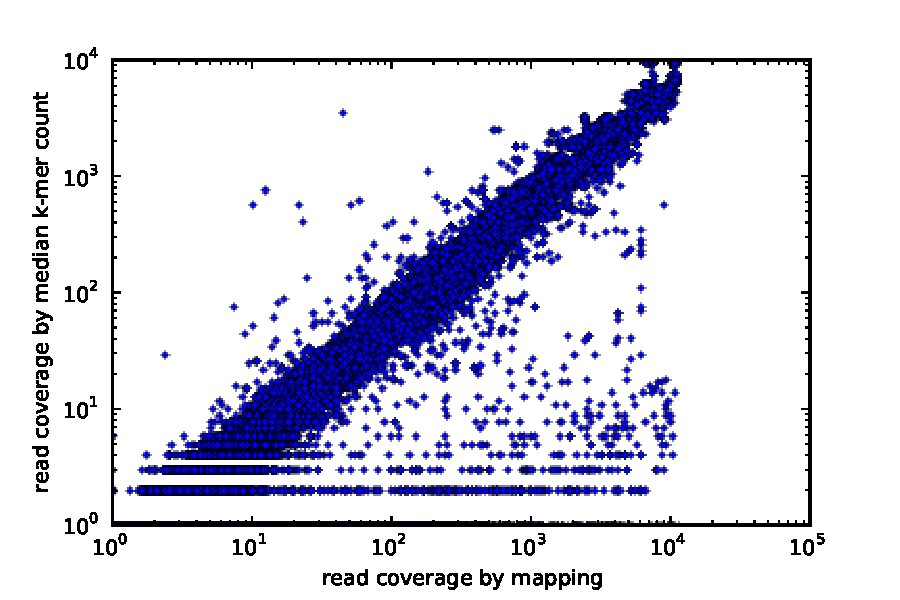
\includegraphics[width=3in]{diginorm-mouse-transcr.pdf}}
\end{center} \caption{ {\bf Mapping and k-mer coverage measures correlate for
simulated transcriptome data as well as real mouse transcriptome data.
Simulated data $r^2 = 0.93$; mouse transcriptome $r^2 = 0.90$.}
}
\label{fig:transcripts} \end{figure}


Using a fixed-memory CountMin Sketch data structure to count k-mers (see
Methods and \cite{countminsketch}), we find that median k-mer abundance
correlates well with mapping-based coverage for artificial and real genomic
data sets.  There is a strong correlation between median k-mer abundance and
mapping-based coverage both for simulated 100-base reads generated with 1\%
error from a 400kb artificial genome sequence ($r^2 = 0.79$; also see Figure
\ref{fig:random}a), as well as for real short-read data from {\em E. coli}
($r^2 = 0.80$, also see Figure \ref{fig:random}b).  This correlation also holds
for simulated and real mRNAseq data: for simulated transcriptome data, $r^2 =
0.93$ (Figure \ref{fig:transcripts}a), while for real mouse transcriptome data,
$r^2 = 0.90$ (Figure \ref{fig:transcripts}b). Thus the median k-mer abundance
of a read correlates well with mapping-based estimates of read coverage.

The coverage on read level estimated from median k-mer count of a read is
always smaller than the mapping-based estimates of read coverage, which is
essentially the coverage on nucleotide level. There is a way to convert the
coverage on read level into real sequencing depth(coverage on nucleotide
level). To cover a k-mer by a read, all the nucleotide in this k-mer must be
covered by the read. If the coverage in nucleotide level is C\_N, the coverage
of a k-mer in a genome will be C\_N * (L-k+1)/L, with length of reads as L.
\cite{Kelley2010} Figure \ref{fig:random} and Figure \ref{fig:transcripts}
shows such relationship obviously.

Such difference between coverage on read level and on nucleotide level is
important in the IGS based diversity analysis method, which will be discussed
in more details in next chapter. For the streaming methods to analyze short
reads data discussed in this chapter, the coverage means the coverage on read
level estimated from median k-mer abundance in a read.



\section{A streaming algorithm to digitally normalize the coverage distribution
of data sets}

Below, we introduce ``digital normalization'', a single-pass lossy compression
algorithm for elimination of redundant reads in data sets based on saturating
coverage of a de Bruijn graph.   While several non-streaming implementations
exist, including Trinity's {\em in silico} normalization
\cite{Haas2013,Brown2012blog}, digital normalization can be efficiently
implemented as a {\em streaming} algorithm.  Critically, no reference sequence
is needed to apply digital normalization.  Digital normalization is inspired by
experimental normalization techniques developed for cDNA library preparation,
in which hybridization kinetics are exploited to reduce the copy number of
abundant transcripts prior to sequencing\cite{pubmed8889548,pubmed7937745}.
{\em Digital} normalization works after sequencing data has been generated,
progressively removing high-coverage reads from shotgun data sets.  This
normalizes average coverage to a specified value, reducing sampling variation
while removing reads, and also removing the many errors contained {\em within}
those reads.  This data and error reduction results in dramatically decreased
computational requirements for {\em de novo} assembly.  This has the advantage
of enabling low-memory preprocessing of both high-coverage genomic data sets,
as well as mRNAseq or metagenomic data sets with high-coverage components
\cite{Brown2012, Howe2012}. Moreover, unlike experimental normalization where
abundance information is removed prior to sequencing, in digital normalization
this information can be recovered from the unnormalized reads.

We present here a fixed-memory implementation of digital normalization that
operates in time linear with the size of the input data.  We then demonstrate
its effectiveness for reducing compute requirements for {\em de novo} assembly
on several real data sets.  These data sets include {\em E. coli} genomic data,
data from two single-cell MD-amplified microbial genomes, and yeast and mouse
mRNAseq.

\subsection{Eliminating redundant reads reduces variation in sequencing depth}

Deeply sequenced genomes contain many highly covered loci.  For example, in a
human genome sequenced to 100x average coverage, we would expect 50\% or more
of the reads to have a coverage greater than 100. In practice, we need many
fewer of these reads to assemble the source locus.

Using the median k-mer abundance estimator discussed above, we can examine each
read in the data set progressively to determine if it is high coverage.  At the
beginning of a shotgun data set, we would expect many reads to be entirely
novel and have a low estimated coverage.  As we proceed through the data set,
however, average coverage will increase and many reads will be from loci that
we have already sampled sufficiently.

Suppose we choose a coverage threshold $C$ past which we no longer wish to
collect reads. If we only keep reads whose estimated coverage is less than $C$,
and discard the rest, we will reduce the average coverage of the data set to
$C$.  This procedure is algorithmically straightforward to execute: we examine
each read's estimated coverage, and retain only those whose coverage is less
than $C$. The following pseudocode provides one approach: 
\begin{verbatim}
   for read in dataset:
      if estimated_coverage(read) < C:
         accept(read)
      else:
         discard(read)
\end{verbatim}
\noindent
\noindent 
where accepted reads contribute to the
$\tt estimated\_coverage$ function.  Note that for any data set with an average
coverage $> 2C$, this has the effect of discarding the majority of reads.
Critically, low-coverage reads, especially reads from undersampled regions,
will always be retained.


\begin{figure}[!ht]
\centerline{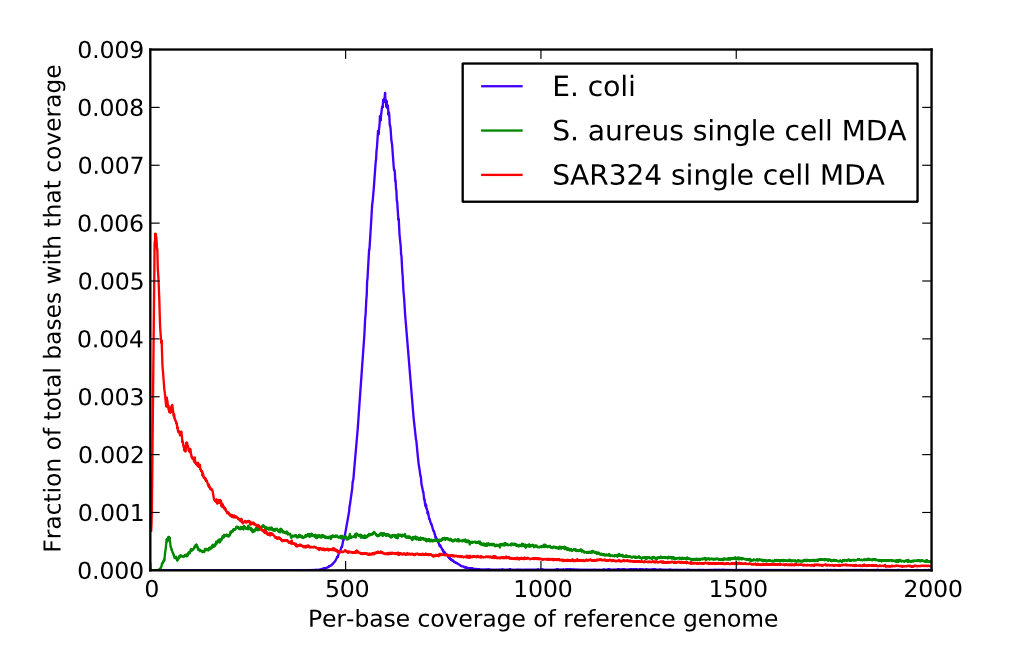
\includegraphics[width=4in]{diginorm-coverage2-raw.png}}
\centerline{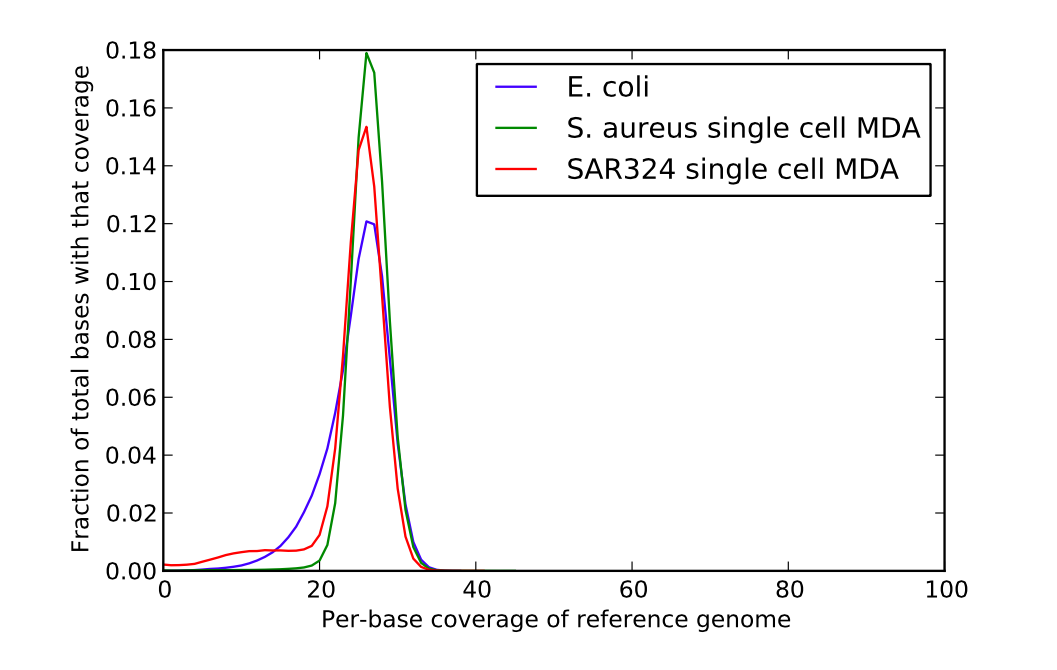
\includegraphics[width=4in]{diginorm-coverage2-dn.png}}
\caption{
{\bf Coverage distribution of three microbial genome samples, calculated
from mapped reads (a) before and (b) after digital normalization (k=20, C=20).}}
\label{fig:coverage}
\end{figure}


The net effect of this procedure, which we call digital normalization, is to
normalize the coverage distribution of data sets.  In Figure
\ref{fig:coverage}a, we display the estimated coverage of an {\em E. coli}
genomic data set, a {\em S. aureus} single-cell MD-amplified data set, and an
MD-amplified data set from an uncultured {\em Deltaproteobacteria}, calculated
by mapping reads to the known or assembled reference genomes (see
\cite{pubmed21926975} for the data source).  The wide variation in coverage for
the two MDA data sets is due to the amplification procedure
\cite{pubmed17487184}.  After normalizing to a k-mer coverage of 20, the high
coverage loci are systematically shifted to an average mapping coverage of 26,
while lower-coverage loci remain at their previous coverage.  This smooths out
coverage of the overall data set.


\begin{figure}[!ht]
\centerline{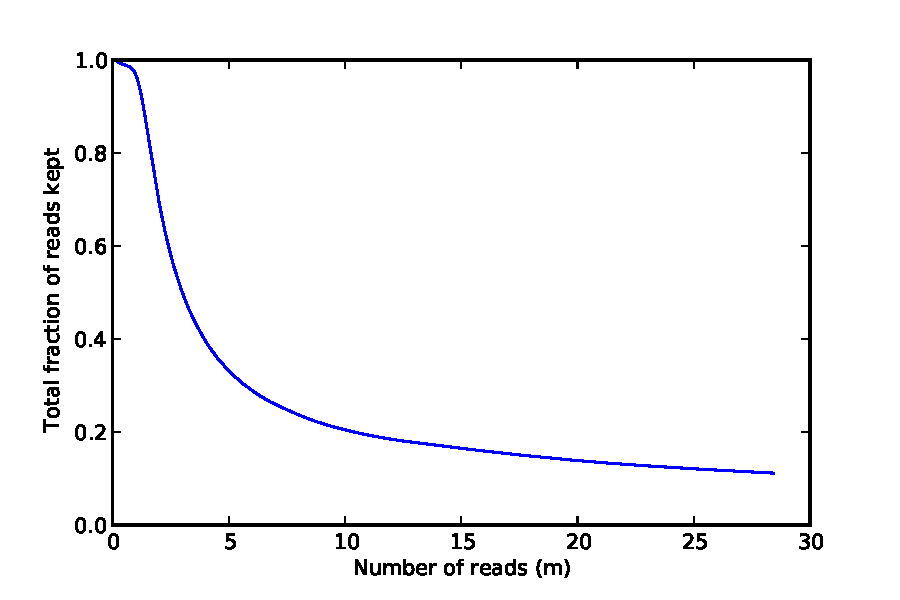
\includegraphics[width=4in]{diginorm-accumulation.pdf}}
\caption{
{\bf Fraction of reads kept when normalizing the {\em E. coli} dataset to C=20 at k=20.}}
\label{fig:accumulate}
\end{figure}


At what rate are sequences retained?  For the {\em E. coli} data set, Figure
\ref{fig:accumulate} shows the fraction of sequences retained by digital
normalization as a function of the total number of reads examined when
normalizing to C=20 at k=20.  There is a clear saturation effect showing that
as more reads are examined, a smaller fraction of reads is retained; by 5m
reads, approximately 50-100x coverage of {\em E. coli}, under 30\% of new reads
are kept.  This demonstrates that as expected, only a small amount of novelty
(in the form of either new information, or the systematic accumulation of
errors) is being observed with increasing sequencing depth.

Here we show that digital normalization provides a general strategy for applying
online or streaming approaches to analysis of {\em de novo} sequencing
data.  The basic algorithm presented here is explicitly a single-pass or streaming
algorithm, in which the entire data set is never considered as a
whole; rather, a partial ``sketch'' of the data set is retained and
used for progressive filtering.  Online algorithms and sketch data
structures offer significant opportunities in situations where data
sets are too large to be conveniently stored, transmitted, or analyzed
\cite{muthukrishnan2005data}.  This can enable increasingly efficient
downstream analyses.
Digital normalization can be applied in any situation where the
abundance of particular sequence elements is either unimportant or can be
recovered more efficiently after other processing, as in assembly, which we will discuss
next.




\subsection{Digital normalization scales assembly of microbial genomes}

We applied the digital normalization and error trimming protocol to
three real data sets from Chitsaz et al (2011) \cite{pubmed21926975}. For all three samples, the number of reads
remaining after digital normalization was reduced by at least 30-fold, while
the memory and time requirements were reduced 10-100x.

%@@(For benchmarking, we used a more recent version of Velvet rather than
%Velvet-SC, because optimizations have been added to Velvet since the Velvet-SC
%fork.)
%
Despite this dramatic reduction in data set size and computational requirements
for assembly, both the {\em E. coli} and {\em S. aureus} assemblies overlapped
with the known reference sequence by more than 98\%.  This confirms that little
or no information was lost during the process of digital normalization;
moreover, it appears that digital normalization does not significantly affect
the assembly results. (Note that we did not perform scaffolding, since the
digital normalization algorithm does not take into account paired-end
sequences, and could mislead scaffolding approaches.  Therefore, these results
cannot directly be compared to those in Chitsaz et al. (2011)
\cite{pubmed21926975}.)

The {\em Deltaproteobacteria} sequence also assembled well, with 98.8\%
sequence overlap with the results from Chitsaz et al. Interestingly, only 30kb
of the sequence assembled with Velvet-SC in Chitsaz et al. (2011) was missing,
while an additional 360kb of sequence was assembled only in the normalized
samples.  Of the 30kb of missing sequence, only 10\% matched via TBLASTX to a
nearby {\em Deltaproteobacteria} assembly, while more than 40\% of the
additional 360kb matched to the same {\em Deltaproteobacteria} sample.
Therefore these additional contigs likely represents real sequence, suggesting
that digital normalization is competitive with Velvet-SC in terms of
sensitivity.

%% @@ better assembly?
%% 
% @ tables or anything?
% 


\begin{table}[!ht]
\caption{
\bf{Single-pass digital normalization to C=20 reduces computational
requirements for transcriptome assembly.}}

%add yeast

\begin{tabular}{|l|c|c|c|c|}

Data set & N reads pre/post & Assembly time pre/post & Assembly memory pre/post \\
 \hline \\
Yeast (Oases) & 100m / 9.3m & 181 min / 12 min (15.1x) & 45.2gb / 8.9gb (5.1x) \\
Yeast (Trinity) & 100m / 9.3m & 887 min / 145 min (6.1x) & 31.8gb / 10.4gb (3.1x) \\
Mouse (Oases) & 100m / 26.4m & 761 min/ 73 min (10.4x) & 116.0gb / 34.6gb (3.4x) \\
Mouse (Trinity) & 100m / 26.4m & 2297 min / 634 min (3.6x) & 42.1gb / 36.4gb (1.2x) \\
\end{tabular}

\begin{flushleft}
\end{flushleft}
\label{tab:dntrans}
\end{table}


\subsection{Digital normalization scales assembly of transcriptomes}


We next applied single-pass digital normalization to published yeast and mouse
mRNAseq data sets, reducing them to 20x coverage at k=20 \cite{pubmed21572440}.
Digital normalization on these samples used 8gb of memory and took about 1 min
per million reads.  We then assembled both the original and normalized sequence
reads with Oases and Trinity, two {\em de novo} transcriptome assemblers (Table
\ref{tab:dntrans}) \cite{pubmed22368243,pubmed21572440}.
%  (Note that
%due to differing execution parameters, the Oases runtimes cannot be directly
%compared to the Trinity runtimes.)
%
For both assemblers the computational resources necessary to complete an
assembly were reduced (Table \ref{tab:dntrans}), but normalization had
different effects on performance for the different samples.  On the yeast data
set, time and memory requirements were reduced significantly, as for Oases
running on mouse.  However, while Trinity's runtime decreased by a factor of
three on the normalized mouse data set, the memory requirements did not
decrease significantly.  This may be because the mouse transcriptome is 5-6
times larger than the yeast transcriptome, and so the mouse mRNAseq is lower
coverage overall; in this case we would expect fewer errors to be removed by
digital normalization.


\begin{table}[!ht]
\caption{
\bf{Digital normalization has assembler-specific effects on transcriptome
assembly.}}

%add yeast

\begin{tabular}{|l|c|c|c|c|}

Data set & Contigs $>$ 300 & Total bp $>$ 300 & Contigs $>$ 1000 & Total bp $>$ 1000 \\
\hline \\
Yeast (Oases) & 12,654 / 9,547 & 33.2mb / 27.7mb & 9,156 / 7,345 & 31.2mb / 26.4mb \\
Yeast (Trinity) & 10,344 / 12,092 & 16.2mb / 16.5mb & 5,765 / 6,053 & 13.6 mb / 13.1mb \\
Mouse (Oases) & 57,066 / 49,356 & 98.1mb / 84.9mb & 31,858 / 27,318 & 83.7mb / 72.4mb \\
Mouse (Trinity) & 50,801 / 61,242 & 79.6 mb / 78.8mb & 23,760 / 24,994 & 65.7mb / 59.4mb \\

\end{tabular}

\begin{flushleft}
\end{flushleft}
\label{tab:dntrans0}
\end{table}


The resulting assemblies differed in summary statistics (Table
\ref{tab:dntrans0}).  For both yeast and mouse, Oases lost 5-10\% of total
transcripts and total bases when assembling the normalized data.  However,
Trinity {\em gained} transcripts when assembling the normalized yeast and mouse
data, gaining about 1\% of total bases on yeast and losing about 1\% of total
bases in mouse.  Using a local-alignment-based overlap analysis (see Methods)
we found little difference in sequence content between the pre- and post-
normalization assemblies: for example, the normalized Oases assembly had a
98.5\% overlap with the unnormalized Oases assembly, while the normalized
Trinity assembly had a 97\% overlap with the unnormalized Trinity assembly.

To further investigate the differences between transcriptome assemblies caused
by digital normalization, we looked at the sensitivity with which long
transcripts were recovered post-normalization.  When comparing the normalized
assembly to the unnormalized assembly in yeast, Trinity lost only 3\% of the
sequence content in transcripts greater than 300 bases, but 10\% of the
sequence content in transcripts greater than 1000 bases.  However, Oases lost
less than 0.7\% of sequence content at 300 and 1000 bases.  In mouse, we see
the same pattern. This suggests that the change in summary statistics for
Trinity is caused by fragmentation of long transcripts into shorter
transcripts, while the difference for Oases is caused by loss of splice
variants.  Indeed, this loss of splice variants should be expected, as there
are many low-prevalence splice variants present in deep sequencing data
\cite{pubmed21151575}. Interestingly, in yeast we recover {\em more}
transcripts after digital normalization; these transcripts appear to be
additional splice variants.

% @table of splice foo?



\begin{table}[!ht]
\caption{
\bf{Digital normalization to C=20 removes many erroneous k-mers from sequencing data sets.  Numbers
in parentheses indicate number of true k-mers lost at each step, based on reference.}}
\begin{tabular}{|l|c|c|c|c|c|}
Data set & True 20-mers & 20-mers in reads & 20-mers at C=20 & \% reads kept\\
\hline \\
Simulated genome & 399,981 & 8,162,813 & 3,052,007 (-2) & 19\% \\
Simulated mRNAseq & 48,100 & 2,466,638 (-88) & 1,087,916 (-9) & 4.1\% \\
{\em E. coli} genome & 4,542,150 & 175,627,381 (-152) & 90,844,428 (-5) & 11\% \\
Yeast mRNAseq & 10,631,882 & 224,847,659 (-683) & 10,625,416 (-6,469) & 9.3\% \\
Mouse mRNAseq & 43,830,642 & 709,662,624 (-23,196) & 43,820,319 (-13,400) & 26.4\% \\
\end{tabular}
\begin{flushleft}
\end{flushleft}
\label{tab:normC20}
\end{table}

\begin{table}[!ht]
\caption{
\bf{Three-pass digital normalization removes most erroneous k-mers.  Numbers
in parentheses indicate number of true k-mers lost at each step, based on known reference.}}
\begin{tabular}{|l|c|c|c|c|}
Data set & True 20-mers & 20-mers in reads & 20-mers remaining & \% reads kept\\
\hline \\
Simulated genome & 399,981 & 8,162,813 & 453,588 (-4) & 5\% \\
Simulated mRNAseq & 48,100 & 2,466,638 (-88) & 182,855 (-351) & 1.2\% \\
{\em E. coli} genome & 4,542,150 & 175,627,381 (-152) & 7,638,175 (-23) & 2.1\% \\
Yeast mRNAseq & 10,631,882 & 224,847,659 (-683) & 10,532,451 (-99,436) & 2.1\% \\
Mouse mRNAseq & 43,830,642 & 709,662,624 (-23,196) & 42,350,127 (-1,488,380) & 7.1\% \\
\end{tabular}
\begin{flushleft}
\end{flushleft}
\label{tab:normC5}
\end{table}

% 
The difference between Oases and Trinity results show that Trinity is more
sensitive to digital normalization than Oases: digital normalization seems to
cause Trinity to fragment long transcripts. Why?  One potential issue is that
Trinity only permits k=26 for assembly, while normalization was performed at
k=20; digital normalization may be removing 26-mers that are important for
Trinity's path finding algorithm.  Alternatively, Trinity may be more sensitive
than Oases to the change in coverage caused by digital normalization.
Regardless, the strong performance of Oases on digitally normalized samples, as
well as the high retention of k-mers (Table \ref{tab:normC20}) suggests that
the primary sequence content for the transcriptome remains present in the
normalized reads, although it is recovered with different effectiveness by the
two assemblers.


\subsection{lower bound on memory usage for effective digital normalization}

In this section, we will discuss the lower bound on memory usage for effective digital
normalization and the effects of high false positive rates particularly.

\begin{table}[!ht]
\caption{ \bf{Low-memory digital normalization. The results of
    digitally normalizing a 5m read {\em E. coli} data set (1.4 GB) to C=20
    with k=20 under several memory usage/false positive rates.  The
    false positive rate (column 1) is empirically determined.  We
    measured reads remaining, number of ``true'' k-mers missing from
    the data at each step, and the number of total k-mers remaining.
    Note: at high false positive rates, reads are erroneously removed due to
    inflation of k-mer counts.}}
\begin{tabular}{ | c | c | c | c | c | c | c |}
\hline
memory   & FP rate & retained reads & retained reads \% & true k-mers missing & total k-mers \\
\hline
before diginorm   &  -      & 5,000,000   & 100.0\%    & 170  &  41.6m \\
2400 MB           &   0.0\% & 1,656,518   &  33.0\%    & 172  &  28.1m \\
240 MB            &   2.8\% & 1,655,988   &  33.0\%    & 172  &  28.1m \\
120 MB            &  18.0\% & 1,652,273   &  33.0\%    & 172  &  28.1m \\
60 MB             &  59.1\% & 1,633,182   &  32.0\%    & 172  &  27.9m \\
40 MB             &  83.2\% & 1,602,437   &  32.0\%    & 172  &  27.6m \\
20 MB             &  98.8\% & 1,460,936   &  29.0\%    & 172  &  25.7m \\
10 MB             & 100.0\% & 1,076,958   &  21.0\%    & 185  &  20.9m \\
\end{tabular}
\begin{flushleft}
\end{flushleft}
\label{table:loop_norm}
\end{table}

\begin{table}[!ht]
\caption{
\bf{{\em E. coli} genome assembly after low-memory digital normalization.
  A comparison of assembling reads digitally normalized with low memory/high
  false positive rates.  The reads were digitally normalized to 
  C=20 (see
  \cite{Brown2012} for more information) and were assembled using Velvet.
  We measured total length of assembly,
  as well as percent of true MG1655 genome covered by the assembly using QUAST.}}
\begin{tabular}{ | c | c | c | c | c | c |}
\hline
memory   & FP rate & N contigs & total length(bases) & \% of true genome covered \\
\hline
before diginorm  &-   & 106 & 4,546,051 & 97.84\% \\
    2400 MB  &  0.0\% & 617 & 4,549,235 & 98.05\% \\
     240 MB  &  2.8\% &  87 & 4,549,253 & 98.04\% \\
     120 MB  & 18.0\% &  86 & 4,549,335 & 98.04\% \\
      60 MB  & 59.1\% &  90 & 4,548,619 & 98.03\% \\
      40 MB  & 83.2\% &  89 & 4,550,599 & 98.11\% \\
      20 MB  & 98.8\% &  85 & 4,550,014 & 98.04\% \\
      10 MB  &100.0\% &  97 & 4,545,871 & 97.97\% \\
\end{tabular}
\begin{flushleft}
\end{flushleft}
\label{table:assembly}
\end{table}

We applied digital normalization to the {\em E. coli} data set used above, and
chose seven different Count-Min Sketch sizes to yield seven different false
positive rates \ref{table:loop_norm}.  The data set was normalized to a k-mer
coverage of 20 and the resulting data were evaluated for retention of true and
erroneous k-mers, as in \cite{Brown2012} (Table \ref{table:loop_norm}).  The
results show that digital normalization retains the same set of underlying
``true'' k-mers until the highest false positive rate of 100\% (Table
\ref{table:loop_norm}, column 5), while discarding only about 2\% additional
reads (Table \ref{table:loop_norm}, column 6).

To evaluate the effect of digital normalization with high false positive rates
on actual genome assembly, we next performed normalization to a coverage of 20
with the same range of false positive rates as above.  We then assembled this
data with Velvet \cite{Zerbino2008} and compared the resulting assemblies to
the known {\em E. coli} MG1655 genome using QUAST (Table \ref{table:assembly}).
To our surprise, we found that even after executing digital normalization with
a false positive rate of 83.2\%, a nearly complete assembly was generated.  No
progressive increase in misassemblies (measured against the real genome with
QUAST) was seen across the different false positive rates (data not shown).
This suggests that below 83.2\% FP rate, the false positive rate of digital
normalization has little to no effect on assembly quality with Velvet.  (Note
that the Velvet assembler itself used considerably more memory than digital
normalization.)

%@CTB quast ref
%
While these results are specific to Velvet and the coverage parameters used in
digital normalization, they do suggest that no significant information loss
occurs due to false positive rates below 80\%. Further evaluation of assembly
quality in response to different normalization parameters and assemblers is
beyond the scope of of this paper.


\subsection{Digital normalization dramatically scales {\em de novo} assembly}

The results from applying digital normalization to read data sets prior to {\em
de novo} assembly are extremely good: digital normalization reduces the
computational requirements (time and memory) for assembly considerably, without
substantially affecting the assembly results.  It does this in two ways: first,
by removing the majority of reads without significantly affecting the true
k-mer content of the data set. Second, by eliminating these reads, digital
normalization also eliminates sequencing errors contained within those reads,
which otherwise would add significantly to memory usage in assembly
\cite{pubmed21245053}.

Digital normalization also lowers computational requirements by eliminating
most repetitive sequence in the data set. Compression-based approaches to graph
storage have demonstrated that compressing repetitive sequence also effectively
reduces memory and compute requirements \cite{pubmed22139935,pubmed22156294}.
Note however that {\em eliminating} many repeats may also have its negatives
(discussed below).

Digital normalization should be an effective preprocessing approach for most
assemblers.  In particular, the de Bruijn graph approach used in many modern
assemblers relies on k-mer content, which is almost entirely preserved by
digital normalization (see Tables \ref{tab:normC20} and \ref{tab:normC5})
\cite{pubmed20211242}.




\section{A streaming algorithm to analyze and trim errors in short reads .}


K-mer spectral analysis is a powerful approach to error detection and
correction in shotgun sequencing data that uses k-mer abundances to
find likely errors in the data \cite{Pevzner2001,Li2003}. 
 The essential idea
is that low-abundance k-mers contained in a high-coverage data set typically
represent random sequencing errors.
A variety of read trimming and error correcting tools use k-mer counting to
reduce the error content of the read data set, independent of quality scores or
reference genomes \cite{Kelley2010}. 

Approaches derived
from spectral analysis can be very effective: spectral error
correction achieves high accuracy, and later we will show that
spectral k-mer trimming is considerably more effective at removing
errors than quality score-based approaches.
However, spectral analysis is also very
compute intensive: most implementations count all the k-mers in
sequencing data sets, which can be memory- or I/O-intensive for large
data sets.

In the section above, we discussed a streaming algorithm for downsampling
read data sets to normalize read coverage spectra, termed ``digital
normalization''.  This procedure
estimates the k-mer coverage of each read in a stream using an online
algorithm. Reads above a certain estimated coverage are set aside and
their k-mers are not tracked.  The diginorm algorithm only examines
the data once, and counts only the k-mers in retained reads, leading
to sublinear memory usage for high-coverage data sets

Here we introduce a semi-streaming algorithm for k-mer spectral
analysis, based on digital normalization, that can detect and remove
errors in sequencing reads.  This algorithm operates in sublinear
memory with respect to the input data, and examines the data at most
twice.  The approach offers a general framework for streaming sequence
analysis and could be used for error correction and variant calling.
Moreover, the approach can be applied generically to data sets with
variable sequencing coverage such as transcriptomes, metagenomes, and
amplified genomic DNA.  We also provide a fully streaming approach for
estimating per-position sequencing error rates in reads that operates
in fixed memory and only examines part of the input data.


\subsection{Two-pass non-streaming method to enable read error analysis}

Firstly, we implemented a two-pass non-streaming method to trim read based on
the new efficient k-mer counting approach we introduced in last chapter. 
Basically in the first pass all the reads in a data set is loaded and the counts of each k-mer are
stored in the Count-Min Sketch. Then during the second pass, for each read, the 
count of every k-mer in it will be examined, if a k-mer with a count as 1 in the 
whole data set is detected, an sequencing error is detected and
the read will be truncated from this k-mer to the end.
In this experiment, we especially evaluated the effect of false-positive induced miscounts on read
trimming.
Because the Count-Min Sketch never undercounts k-mers, reads will never be
erroneously trimmed at truly high-abundance k-mers; however, reads may not be
trimmed correctly when miscounts inflate the count of low-abundance k-mers.  In
cases where many errors remain, read trimming can potentially be applied
multiple times, with each round reducing the total number of k-mers and hence
resulting in lower false positive rates for the same memory usage.

\begin{table}[!ht]
\caption{
\bf{Iterative low-memory k-mer trimming.  The results of trimming
  reads at unique (erroneous) k-mers from a 5m read {\em E. coli} data set (1.4 GB)
  in under 30 MB of RAM.  After each iteration, we measured the
  total number of distinct k-mers in the data set, the total number
  of unique (and likely erroneous) k-mers remaining, and the
  number of unique k-mers present at the 3' end of reads.}}
\begin{tabular}{ | c | c | c | c | c | c |}
\hline
 & FP rate & bases trimmed & distinct k-mers & unique k-mers & 
unique k-mers at 3' end \\
\hline
untrimmed                           &      -  &      - & 41.6m & 34.1m & 30.4\%  \\
khmer iteration 1                   & 80.0\%  & 13.5\% & 13.3m &  6.5m & 29.8\% \\
khmer iteration 2                   & 40.2\%  &  1.7\% &  7.6m & 909.9k & 12.3\% \\
khmer iteration 3                   & 25.4\%  &  0.3\% &  6.8m & 168.1k & 3.1\% \\
khmer iteration 4                   & 23.2\%  &  0.1\% &  6.7m &  35.8k & 0.7\% \\
khmer iteration 5                   & 22.8\%  &  0.0\% &  6.6m &   7.9k & 0.2\% \\
khmer iteration 6                   & 22.7\%  &  0.0\% &  6.6m &   1.9k & 0.0\% \\
filter by FASTX                     &      -  &  9.1\% & 26.6m & 20.3m & 26.3\% \\
filter by seqtk(default)            &      -  &  8.9\% & 17.7m & 12.1m & 12.3\% \\
filter by seqtk(-q 0.01)            &      -  & 15.4\% &  9.9m &  5.1m &  5.2\% \\
filter by seqtk(-b 3 -e 5)          &      -  &  8.0\% & 34.5m & 27.7m & 25.3\% \\
\end{tabular}
\begin{flushleft}
\end{flushleft}
\label{table:loop_trim}
\end{table}


We performed six iterations of unique k-mer trimming on 5 million Illumina
reads from sequencing of {\em E. coli}, with memory usage less than 30 MB.  For
each iteration we measured empirical false positive rate compared with number
of bases trimmed as well as the total number of k-mers (Table
\ref{table:loop_trim}).  In the first round, the estimated false positive rate
was 80.0\%, and 13.5\% of the total bases were removed by trimming reads at
low-abundance k-mers; the second iteration had a false positive rate of 37.7\%,
and removed only 1.5\% additional data; and by the fourth iteration the false
positive rate was down to 23.2\% with 0.0\% of the data removed.

The elimination of so many unique k-mers (column 5) in the first pass was
unexpected: the high false positive rate should have resulted in fewer k-mers
being identified as unique, were the erroneous k-mers independent of each
other. Upon examination, we realized that in Illumina data erroneous k-mers
typically come from substitution errors that yield runs of up to k erroneous
k-mers in a row \cite{Kelley2010}.  When trimming reads with high false
positive rates, these runs are typically trimmed after the first few unique
k-mers, leaving unique k-mers at the 3' end.  Because of this we hypothesized
that high-FP rate trimming would result in the retention of many unique k-mers
at the 3' end of the read, and this was confirmed upon measurement (Table
\ref{table:loop_trim}, column 6, pass 1 vs pass 2).

In comparison to quality-based trimming software such as seqtk and FASTX,
trimming at unique k-mers performed very well: in this data set, all unique
k-mers represent errors, and even with an initial false positive rate of 80\%,
khmer outperformed all but the most stringent seqtk run (Table
\ref{table:loop_trim}).  With a lower false positive rate or multiple passes,
khmer eliminates more erroneous k-mers than seqtk or FASTX.  The tradeoff here
is in memory usage: for larger data sets, seqtk and FASTX will consume the same
amount of memory as on smaller data sets, while khmer's memory usage will need
to grow with the data set size.


With Illumina sequencing, average and per-position error rates may
vary between sequencing runs, but are typically systematic within a
run \cite{drisee}.  Melsted and Halldorson (2014) introduced an
efficient streaming approach to estimating per-run sequencing error,
but this approach does not apply to error rates by position within
reads \cite{Melsted2014}.  Here, k-mer spectral error analysis can be
used to calculate per-position relative sequencing error for entire
data sets. 


\begin{figure}[!ht]
\centerline{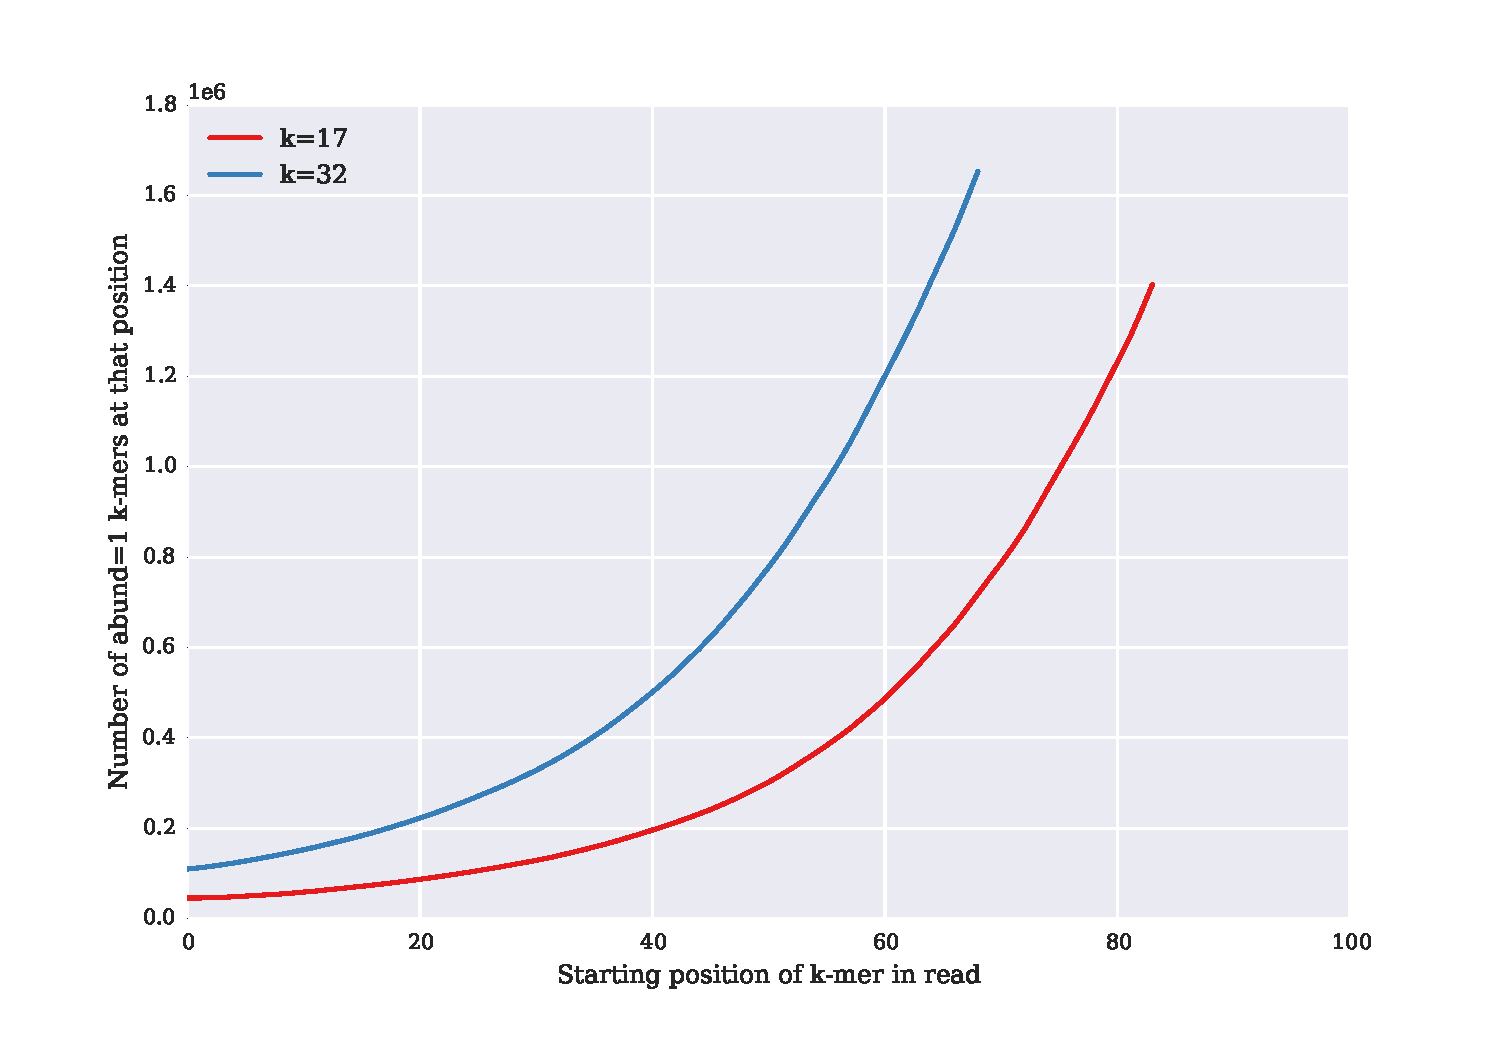
\includegraphics[width=5in]{./figures/figure7_perc_unique_pos}}
\caption{\bf Number of unique k-mers (y axis) by starting position within read
(x axis) in an untrimmed {\em E. coli} 100-bp Illumina shotgun data set, for
k=17 and k=32.  The increasing numbers of unique k-mers are a sign of the
increasing sequencing error towards the 3' end of reads.  Note that there are
only 69 starting positions for 32-mers in a 100 base read.}
\label{fig:perc_unique_pos} \end{figure}



In Figure \ref{fig:perc_unique_pos}, we use khmer to examine the sequencing
error pattern of a 5m-read subset of an Illumina reads data set from
single-colony sequencing of {\em E. coli} \cite{pubmed21926975}.  The high rate
of occurrence of unique k-mers close to the 3' end of reads is due to the
increased sequencing error rate at the 3' end of reads.


The results above demonstrated that the newly developed 
k-mer counting approach can be integrated successfully to do effective error 
analysis. This is an application where the counting error of the Count-Min Sketch approach
used by khmer may be particularly tolerable: it will never falsely
call a high-abundance k-mer as low-abundance because khmer never
underestimates counts.



\subsection{A semi-streaming algorithm can be used for error analysis}



As shown above, k-mer spectral error detection, trimming, and correction approaches
are typically implemented as a two-pass offline algorithm, , in which
k-mer counts are collected in a first pass and then reads are
analyzed in a second pass.  While several algorithms that run in
sublinear memory do exist (e.g., Lighter \cite{lighter}), these are
still offline algorithms that require two or more passes across
the data.



In high coverage data sets it is possible to implement a more
algorithmically efficient approach, by detecting reads that are high
coverage in the context of reads previously encountered in the same
pass of the data. 
Shotgun sequencing oversamples most regions -- for example, for a 100x
coverage genomic data set, we would expect 50\% or more of the genome
to be represented by more than 100 reads.  This is a consequence of
the Poisson-random sampling that underlies shotgun sequencing
\cite{waterman}.  This oversampling provides an opportunity, however:
if we regard the read data set as a stream of incoming data randomly
sampled from a pool of molecules, high-abundance species or
subsequences within the pool will be more highly sampled in the stream
than others, and will thus generally appear earlier in the stream.
For example, in mRNAseq, highly expressed transcripts should almost
always be sampled much more frequently than low-expressed transcripts,
and so more reads from highly expressed transcripts will be seen in
any given subset.With this in mind, we can develop an approach to do 
{\em semi-streaming} error analysis by detecting and
analyzing high-coverage reads {\em during} the first pass. 

We implemented this by integrating k-mer spectral
error analysis directly into the digital normalization algorithm.
As digital normalization, here we
still use the median k-mer abundance of the k-mers in a read to
estimate that read's abundance \cite{Brown2012}; crucially, this can
be done at any point in a stream, by using the online k-mer counting
functionality of khmer to determine the abundance of k-mers seen thus
far in the stream \cite{Zhang2014}. 


\begin{figure}[!ht]
 \centerline{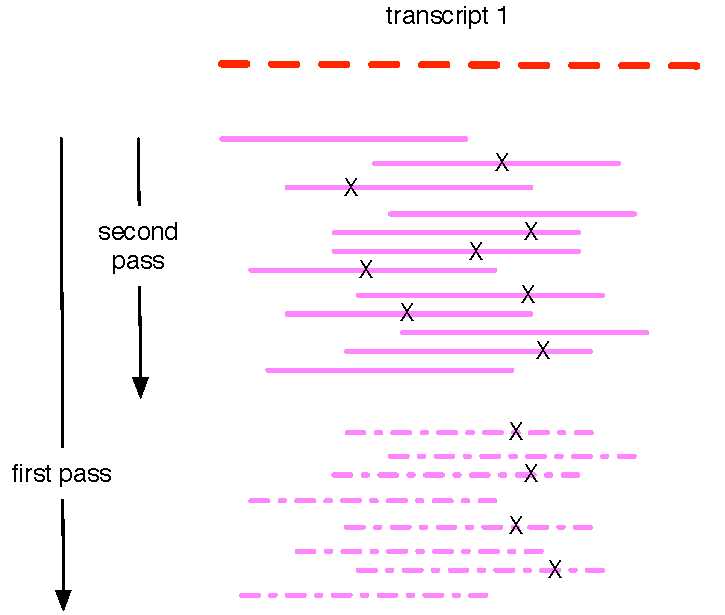
\includegraphics[width=4in]{./figures/graph-saturation}}
\caption{\bf Diagram of semi-streaming error detection. In a first pass
over the read data, reads are loaded in until the graph locus to which
they belong is saturated.  From that point on, reads are examined for
errors and not loaded into the graph.  In a second pass, only the subset
of reads loaded into the graph are examined for errors.}
\label{fig:concept}
\end{figure}

The conceptual idea is presented in Figure~\ref{fig:concept}.  On the
first pass, low-coverage reads would be incorporated into the k-mer
database with all the k-mers in them loaded into memory, and set aside for later analysis, because we can not reliably detect error, which 
is a low-abundance k-mer in a low-coverage read. 
Meanwhile, the high-coverage reads
would be analyzed for errors but would not be incorporated into the k-mer database.
This step is similar to digital normalization where the high-coverage reads are
discarded. Not loading the k-mers in those high-coverage reads decreases the
counts of those high abundance k-mers in the k-mer database a bit but this
does not affect the counts of those low abundance k-mers. So this process will
not influence the detection of errors. 
Actually the special treatment to high coverage reads also dismisses many errors in
those high coverage reads 
and this makes the detection of low abundance k-mers more accurate.

On the second pass, the set aside reads which were considered as low-coverage reads
would be checked for coverage again, and either ignored or analyzed
for errors.  Crucially, this second pass involves {\em at most}
another full pass across the data, but only when the entire data set
is below the coverage threshold; the larger the high coverage
component of the data, the smaller the fraction of the data that is
examined twice.


In Figure~\ref{fig:saturation}, we show diginorm-generated coverage
saturation curves for both real and error-free simulated reads from
{\em E. coli} MG1655.  In both cases, after the first 1m reads, the
majority of reads have an estimated coverage of 20 or higher, and
hence can be used for error analysis on the remainder of the data
encountered in the first pass.

\begin{figure}[!ht]
 \centerline{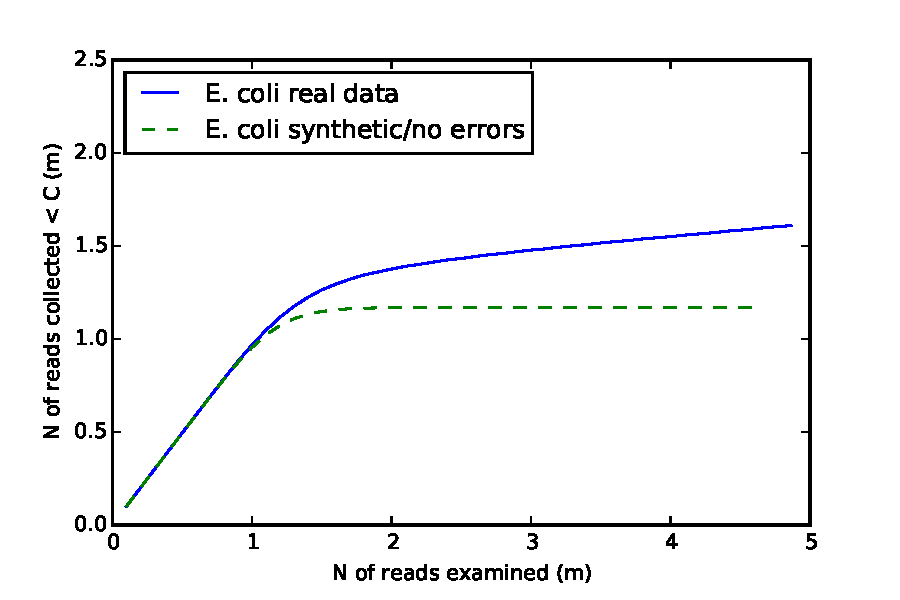
\includegraphics[width=4in]{./figures/saturation}}
\caption{\bf Saturation curve of a real and a simulated {\em E. coli}
  read data set.  Reads are collected when they have an estimated
  coverage of less than 20; in the early phase ($<$ 1m reads), almost
  all reads are collected, but by 2m reads into the data set, the
  majority of reads come from loci with an estimated sequencing depth
  of $>$ 20 and are rejected.}
\label{fig:saturation}
\end{figure}


The algorithm for the {\em semi-streaming} analysis of reads can be described as
follows:
\begin{verbatim}
for read in data:  # first pass
   if estimated_coverage(read) < C:
      count_kmers(read, k-mer_database) #
      save(read)
   else:
      analyze(read)

for read in saved_reads:   # second pass
   if estimated_coverage(read) >= C:
      analyze(read)
\end{verbatim}


As with digital normalization, a basic semi-streaming approach is very
simple to implement: with an online way to count k-mers, the algorithm
is approximately 10 lines of Python code.  The approach also requires
very few parameter choices: the only two parameters are k-mer size and
target coverage C.  However, we do not yet know how these parameters
interact with read length, error rate, or data set coverage;
systematic evaluation of parameters and the development of underlying
theory is left for future work.  In practice, we expect that
additional work will need to be done to adapt existing error
correction approaches to use the semi-streaming approach.



% 
\subsection{Semi-streaming error trimming on synthetic and real data:}

We next adapted the error detection algorithm to do semi-streaming
error trimming on synthetic or real genomic, metagenomic, and transcriptomic data. 

On the synthetic ``simple genome'' this
trimming approach eliminates 149 reads entirely and truncates another 392
reads.  Of the 100,000 bp in the simulated reads, 31,910 (31.9\%) were removed
by the trimming process.  In exchange, trimming eliminated {\em all} of the
errors, bringing the overall error rate from 0.63\% to 0.00\%.

% make mcompare5 make rcompare5
% 
For the synthetic ``simple metagenome'' we only trimmed reads with estimated coverage of 
20 or higher.  Here, of
2347 reads containing 234,700 bp, 314 reads (13.4\%) were removed and 851 reads
(36.3\%) were trimmed, discarding a total of 74,321 bases (31.7\%).  Of 1451
errors total, all but 61 were eliminated, bringing the overall per-base error
rate from 0.62\% to 0.04\%.  The simple mRNAseq data set showed similar
improvement: 83 of 568 reads were removed, and 208 were trimmed, removing
19,507 of 56,800 bases (34.34\%).  The initial error rate was 0.65\% and the
final error rate was 0.07\%. 



% ecoli-report-untrim.txt ('make ecoli-report-untrim.txt')
%posfile ecoli-reads.sam.pos: 2177509 mutated reads of 4960248; 7990149
%mutations total 496024800 bp total overall error rate: 1.610837%
%
% ecoli-report-trim.txt ('make ecoli-report-trim.txt')
%posfile ecoli-abundtrim.sam.pos: 164655 mutated reads of 4861345; 203345
%mutations total 434621201 bp total overall error rate: 0.046787%
%
% output of 'make ecoli-mapped.fq.gz.abundtrim'
% % % %
% read 4960248 reads, 496024800 bp wrote 4861345 reads, 434621201 bp removed
% 98903 reads and trimmed 2030456 reads trimmed or removed 12.38% of bases
% (61403599 total) fp rate estimated to be 0.004
% 
Applying the semi-streaming error trimming to the {\em E. coli} MG1655 data
set, we trimmed 2.0m reads and removed 50,281 reads entirely.  Of 8.0m errors,
all but 203,345 were removed, bringing the error rate from 1.49\% to 0.07\%.
Trimming discarded 53 Mbp of the original 486 Mbp (11.1\%).

% rseq_compare5.txt rseq_compare5b.txt
% 
% make podar_compare5
% 
On the mouse mRNAseq data set, semi-streaming error trimming removed 919,327
reads and trimmed 648,322 reads, removing 19.8\% of the total bases, bringing
the overall error rate from 1.59\% to 1.21\%.  When we measured only the error
rate in the high-coverage reads, trimming brought the error rate from 1.20\% to
0.42\%.  On the mock metagenome data set, 27,554 reads were removed and 171,705
reads were trimmed, removing 0.36\% of bases; this low percentage is because of
the very low coverage of most of the reads in this data set.



% ecoli-report-untrim.txt, ecoli-report-trim.txt
% rseq_compare5.txt
% rseq_compare5b.txt
% podar_
% podar_compare5b

\begin{table}
\begin{tabular}{|l|c|c|c|c|}
\hline
Data set        & pre-trim error & \% bp trim & \% reads trim & post-trim error \\
\hline
{\em E. coli}   & 1.49\%         & 11.05\%          & 41.9\%      & 0.07\% \\
\hline
mouse mRNAseq   & 1.59\%         & 13.9\%           & 19.8\%      & 1.21\% \\
(high coverage only) & 1.20\%    & 20.4\%           & 29.0\%      & 0.42\% \\
\hline
Mock metagenome & 0.31\%         & 0.4\%            & 1.1\%       & 0.28\% \\
(high coverage only) & 0.16\%    & 1.4\%            & 3.5\%       & 0.07\% \\
\hline
\end{tabular}

\caption{{\bf A summary of trimming statistics for semi-streaming
    error trimming.  Error rates before and after trimming were
    estimated by mapping. ``High coverage'' numbers refer to the
    subset of reads with $C \geq 20$ that were subject to analysis.}}
\label{tab:trimming}
\end{table}



% cmouse-compare5-post.txt  cpodar-compare5-post.txt
% cmouse-compare5-pre.txt   cpodar-compare5-pre.txt

\begin{table}
\centering
\begin{tabular}{|l|c||c|}
\hline

Data set             & mouse mRNAseq      & mock metagenome \\
\hline
Total reads          & 81.3m         & 103.2m \\
Total bp             & 6.18 Gbp      & 10.4 Gbp \\
High-coverage reads  & 74.6m         & 91.9m \\
Number of passes     & 1.18          & 1.43 \\
\% reads trim        & 25.0\%        & 11.75\% \\
\% bp trim           & 13.74\%       & 4.03\% \\
Pre-trim error rate  & 1.89\%        & 0.27\% \\
Post-trim error rate & 1.30\%        & 0.15\% \\
\hline
\end{tabular}

\caption{{\bf Results of streaming error trimming on complete data sets.
Error rates before and after trimming were estimated by mapping.}}
\label{tab:full_trimming}
\end{table}


In practice, the space and time performance of both digital normalization and
the generalized streaming approach presented here depend on specific details of
the data set under analysis and the precise implementation of the coverage
estimator. While our intention in this paper is to demonstrate the general
streaming approach, we note that even our naive implementation for e.g.
streaming trimming is useful and can be applied to very large data sets.  For
high coverage data, we can efficiently error-trim 10s of millions of reads in
both sublinear memory and fewer than two passes across the data.  In
Table~\ref{tab:full_trimming}, we show the summary statistics for streaming
error trimming of the full mouse mRNAseq and mock metagenome data; in contrast
to the smaller subsets used previously (see Table~\ref{tab:trimming}), when we
consider the full data sets the majority of reads are examined only once (see
``Number of passes'', Table~\ref{tab:full_trimming}).


The implementation of semi-streaming error trimming used here is
somewhat inefficient, and relies on redundantly storing all of the
reads needed for the second pass on disk during the first pass.  In
the worst case, where all reads are low coverage, a complete copy of
the data set may need to be stored on disk!  This is an area for
future improvement.  However, when we look at full data sets, fewer
than half the reads are examined twice (see Number of passes,
Table~\ref{tab:full_trimming}).




\subsection{Semi-streaming Illumina error rates and error profiles analysis}

\begin{figure}[!ht]
 \centerline{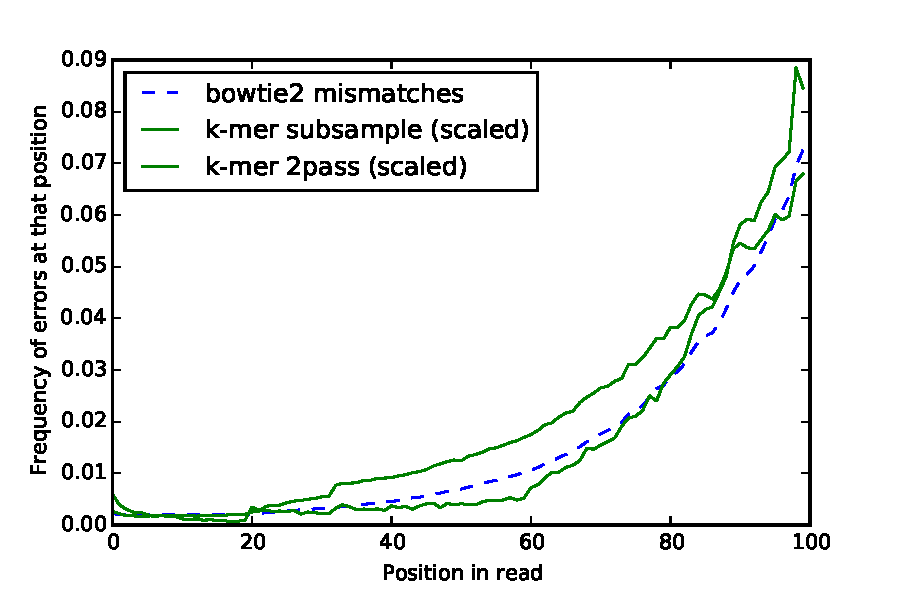
\includegraphics[width=4in]{./figures/ecoli-errhist}}
\caption{{\bf Error spectrum of reads in the {\em E. coli} data
    set. The sublinear k-mer spectrum analysis is calculated based on
    saturation of a fraction of the data set, while the two-pass
    spectral analysis uses all of the data.  bowtie2 mismatches are
    based on all mapped reads.  The y values for the k-mer spectral
    analyses are scaled by a factor of four for ease of comparison.}}
\label{fig:ecoli_err}
\end{figure}

\begin{figure}[!ht]
 \centerline{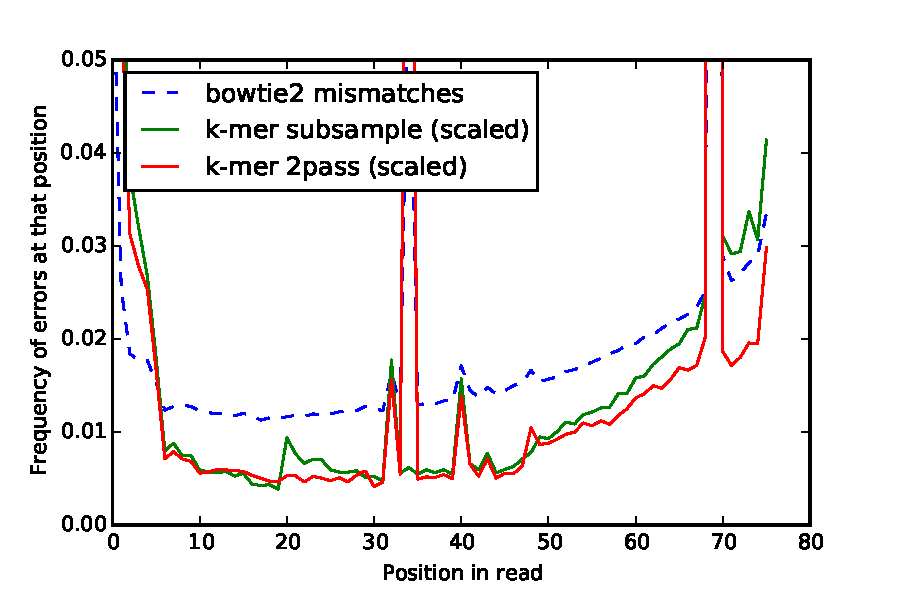
\includegraphics[width=4in]{./figures/rseq-errhist}}
\caption{{\bf Error spectrum of reads in the mouse RNAseq data set.
    The sublinear k-mer spectrum analysis is calculated based on
    saturation of a fraction of the data set, while the two-pass
    spectral analysis uses all of the data, and bowtie2 mismatches are
    based on all mapped reads.  The peak of errors at position 34 in
    the bowtie2 mapping reflects errors that in the first part of the
    data set are called as Ns, and hence are ignored by the sublinear
    error analysis; see text for details. Note, the bowtie2 mismatch
    rates are larger than the spectral rates, so for ease of
    comparison the y values for the k-mer spectral analyses are scaled
    by a factor of four.}}
\label{fig:rseq_err}
\end{figure}



We can adapt the streaming approaches above to efficiently provide estimates
for {\em subsets} of the data.  The basic idea is to consume reads until some
reads have saturated, and then to calculate error rates for new reads from the
saturated loci in the graph.  This can be done in one pass for data sets with
sufficiently high coverage data: as shown above (Figure~\ref{fig:saturation}),
in some data sets, most of the reads will have sufficient coverage to call
errors by the time 20\% of the data set has been consumed.

Using the same error detection code as above, we implemented a sublinear
memory/sublinear time algorithm that collects reads until some regions have
reached 20x coverage, or 200,000 reads have surpassed a coverage of 10x (see
Methods for details).  In either case, all reads at or above a coverage of 10
are analyzed for errors, with a trusted k-mer cutoff of 3.  In
Figure~\ref{fig:ecoli_err} and Figure~\ref{fig:rseq_err} we show the resulting
error profiles for the {\em E. coli} and mouse RNAseq data sets, compared with
the profile obtained by examining the locations of mismatches to the
references. We also show the error profile obtained with the full two-pass
approach (using digital normalization and then error detection as above) for
comparison.

In the {\em E. coli} data set (Figure~\ref{fig:ecoli_err}), we see the increase
in error rate towards the 3' end of the gene that is characteristic of Illumina
sequencing \cite{biases}.  All three error profiles agree in shape (Pearson's
correlation of 0.99 between each pair) although they are offset considerably in
absolute magnitude. The k-mer error profile was calculated from the first
850,000 reads, but is consistent across five other subsets of the data chosen
randomly with reservoir sampling (data not shown); all five subsets had
Pearson's correlation coefficients greater than 0.99 with the bowtie2 mapping
profile and the two-pass spectral approach.

The RNAseq error profile exhibits two large spikes, one at position 34 and one
at position 69.  Both spikes appear to be genuine and correlate with large
numbers of Ns in those positions in the original data set.  The spikes are
present in the profiles derived from two-pass spectral analysis as well as the
bowtie2 mismatch calculation.  However, the sublinear approach does not detect
them when using the first 675,000 reads.  This is because of the choice of
subsample: five other subsamples, chosen randomly from the entire data set with
reservoir sampling, match the match the two-pass spectral analysis (data not
shown).  The error profiles calculated from all six subsamples with the
sublinear algorithm have a Pearson's correlation coefficient greater than 0.96
with the error profiles from the full two-pass spectral approach and the
bowtie2 mismatches.


The ability to analyze high-coverage reads without examining the
entire data set offers some intriguing possibilities.  One concrete
application that we demonstrate here is the use of high coverage reads
to infer data-set wide error characteristics for shotgun data, in a
way that is robust to the sample type \cite{drisee}.  This approach
could also be integrated directly into sequencers to assess whether
the target coverage has been obtained, and perhaps stop sequencing.
More generally, the approach of using saturating coverage to truncate
computational analysis may have application to streaming sequencing
technologies such as SMRT and Nanopore sequencing, where realtime
feedback between sequencing and sequence analysis could be useful
\cite{pacbio,nanopore}.


\section{Time and space usage of the streaming algorithm for analyzing 
short DNA sequencing reads}

As shown above, the essential idea of error analysis generally is that low-abundance
k-mers contained in a high-coverage data set typically represent
random sequencing errors. We address this problem by making use of k-mer spectra, a common
approach in which reads are treated as subpaths through a De
Bruijn graph, and errors in the reads are identified by finding
low-frequency subpaths \cite{Pevzner2001}.  


We generalize this approach by
building the graph with an online algorithm and detecting regions of
the graph saturated by observations.  These regions can then be used
for per-read analysis without necessarily examining the entire data
set.


\paragraph*{Detecting graph saturation:}
We detect graph saturation with digital normalization. The digital
normalization algorithm is, in Python pseudocode:
\begin{verbatim}
for read in data:
   if coverage(read, table) < DESIRED:
      add_read_to_graph(read, graph)
      analyze(read)
\end{verbatim}
This is a single-pass algorithm that can be implemented in fixed space
using a Count-Min Sketch to store the De Bruijn graph necessary for
coverage estimation \cite{Pell2012, Zhang2014}.  For any
error-containing data set with coverage greater than {\tt DESIRED},
the graph requires space less than the size of the input - typically
space sublinear in the data size, for any fixed-size source text (see
Figure~\ref{fig:saturation} and \cite{Zhang2014}).

The digital normalization algorithm was developed as a {\em filter},
in which the reads are passed on to another program (such as a {\em
  de novo} assembler) for further analysis -- these later analyses are
typically based on multi-pass, heavyweight algorithms.  Here, digital
normalization is performing lossy compression, reducing the number of
error-containing sentences while attempting to retain the structure of
the De Bruijn graph \cite{Brown2012, Zhang2014, Lowe2015}.  This reliance
on a post-normalization heavyweight analysis step limits the
applicability of digital normalization and presents challenges in the
analysis of extremely large data sets, which motivated this work.

\paragraph*{Semi-streaming analysis:} The algorithm for {\em semi-streaming} analysis of reads is as
follows:
\begin{verbatim}
for read in data:  # first pass
   if coverage(read, graph) < DESIRED:
      add_read_to_graph(read, graph)
      save(read)
   else:
      analyze(read)

for read in saved_reads:   # second pass
   if coverage(read, graph) >= DESIRED:
      analyze(read)
\end{verbatim}
Here, the space used for the graph remains identical to the digital
normalization algorithm and is typically sublinear in space for high
coverage data sets, but the algorithm is no longer single-pass, and
requires re-examining some subset of the input data in a second pass.
In the worst case scenario, with an undersampled source text (or
randomly generated sentences), this is a fully offline two-pass
approach that requires re-examining {\em all} of the input data for
the second pass.  In practice, most real data sets will require fewer
than two passes: graphically, any deviation from the identity line in
a saturation analysis as in Figure~\ref{fig:saturation} yields a
few-pass algorithm.


\section{Conclusion}



Shotgun DNA sequencing generates data as a stream
of items representing sentences (``reads'') randomly sampled from a
larger text, with replacement. There are several distinct features of this kind
of stream-like data.
 The first is that important details of the source text,
such as its size and statistical composition, may be completely
unknown; that is, often the reads themselves are the most specific
information we have about the source text.  Second, the source text
may be incompletely sampled by the reads, and whether or not it is
completely sampled may not be known in advance.  And third, read
data sets are typically stored on disk, at least in current
implementations; our goal is to identify more efficient approaches to
examining these data sets without necessarily moving to a pure
streaming model, which allows us to make use of the {\em
  semi-streaming} paradigm introduced by Feigenbaum et
al. \cite{Feigenbaum2005}.

 In this chapter, we discussed our solutions to
two primary problems. One is to efficiently distill the non-redundant informaiton
from the streaming to reduce the size of data finally without losing much important 
information. The other one is to
efficiently identify the locations of errors in these reads by
finding differences with respect to the (unknown) source text. Both solutions 
are based on a novel approach to use median k-mer count in a read to estimate
sequencing depth without a reference assembly, which will also be the foundation
of the IGS based diversity analysis method discussed in the next chapter.

Streaming represents the future of big data. 
This kind of problems we are dealing with is not only critically important to 
a better understanding of the exploding big biological data, but also a 
gateway to a larger set of interesting domain problems
dealing with big data, like estimating the true abundance of the 
sentences in the larger text or detecting evil traffic in the internet data
stream.






\section{Data}

The code and detailed instruction used to generate all of the results in this chapter is available at
github.com/ged-lab/2012-paper-diginorm/ and 
http://github.com/ged-lab/2014-streaming/. 

\subsection{Data sets used for digital normalization}

The {\em E. coli}, {\em S. aureus}, and {\em Deltaproteobacteria} data sets
were taken from Chitsaz et al. \cite{pubmed21926975}, and downloaded from
bix.ucsd.edu/projects/singlecell/.  The mouse data set was published by
Grabherr et al. \cite{pubmed21572440} and downloaded from
trinityrnaseq.sf.net/.  All data sets were used without modification. The
complete assemblies, both pre- and post-normalization, for the {\em E. coli},
{\em S. aureus}, the uncultured {\em Deltaproteobacteria}, mouse, and yeast
data sets are available from ged.msu.edu/papers/2012-diginorm/.

The simulated genome and transcriptome were generated from a uniform AT/CG
distribution.  The genome consisted of a single chromosome 400,000 bases in
length, while the transcriptome consisted of 100 transcripts of length 500.
100-base reads were generated uniformly from the genome to an estimated
coverage of 200x, with a random 1\% per-base error.  For the transcriptome, 1
million reads of length 100 were generated from the transcriptome at relative
expression levels of 10, 100, and 1000, with transcripts assigned randomly with
equal probability to each expression group; these reads also had a 1\% per-base
error.


\subsection{Synthetic data sets used for error analysis}

We computationally constructed three small short-read DNA data sets for initial
exploration of ideas.  All synthetic sequences have equiprobable A/C/G/T.  All
synthetic reads are 100bp long and were sampled with 1\% error.  The ``simple
genome'' data set consists of 1000 reads chosen uniformly from a 1 kb randomly
constructed genome. The ``simple transcriptome'' data set consists of 568 reads
chosen uniformly from synthetic transcripts containing different subsets of
four 250-base exons, with expression levels varying by a factor of 30 from
minimum to maximum.  The ``simple metagenome'' data set consists of reads
sampled from three different 500 bp sequences, across 30 fold variation in
abundance.  In all three cases, the errors during read sampling were recorded
for comparison with predictions.

\subsection{Real data sets used for error analysis}

We used three shotgun Illumina data sets: a genomic data set from {\em E.
coli}, a mRNAseq data set from {\em Mus musculus}, and a mock community
metagenome.  For {\em E. coli}, we took a 5m read subset of ERA000206 from
\cite{chitsaz}.  For mRNAseq, we used a 10m read subset of GSE29209 from
\cite{trinityrna}.  For the mock metagenome, we used a 20m read subset of
SRR606249 from \cite{podar}.  Prior to analysis, we eliminated any read with an
'N' in it and filtered the reads by mapping to the known references, yielding
the read numbers in Table~\ref{tab:data}.

